\documentclass{article}

% Paquets nécessaires
\usepackage{amsmath} % Pour les mathématiques
\usepackage{amsfonts} % Pour les polices mathématiques supplémentaires
\usepackage{amssymb} % Pour les symboles mathématiques
\usepackage{tikz} % Pour les graphiques vectoriels
\usepackage{pgfplots} % Pour les graphiques en 2D et 3D
\usepackage{setspace} % Pour l'espacement des lignes
\usepackage{color} % Pour les couleurs de texte
\usepackage{mathrsfs} % Pour les lettres cursives en mathématiques
\usepackage{blindtext}
\usepackage{pdflscape}
\usepackage{adjustbox}
\usepackage{geometry}

\usetikzlibrary{automata, positioning, arrows}
% Configuration des bibliothèques TikZ
\usepgfplotslibrary{fillbetween}
\pgfplotsset{compat=1.18}
\begin{document}
\newgeometry{
    top=3cm,
    bottom=3cm,
    left=6cm,
    right=4cm,
}
\begin{landscape}
   \begin{center}
        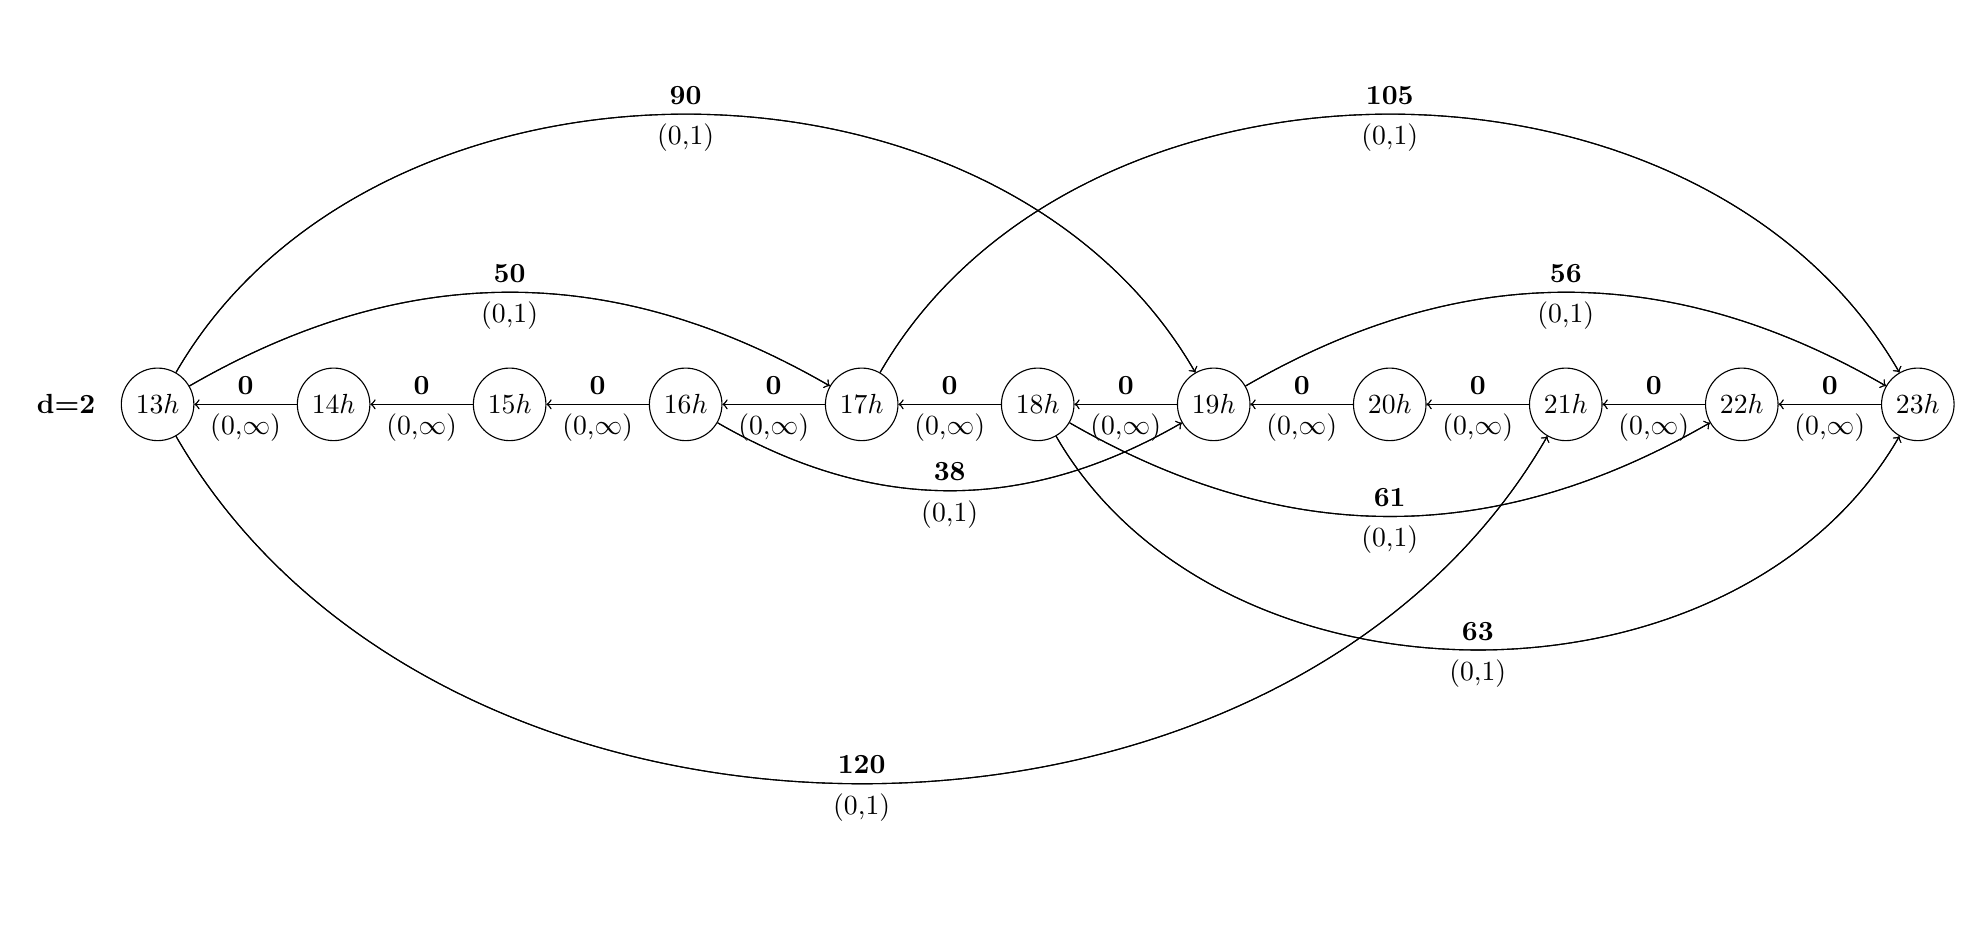
\begin{tikzpicture}[node distance=1.3cm,auto]
            \tikzset{label/.style={midway,font=\small}}

            \node[state] (13h) {$13h$};
            \node[state] (14h) [right = of 13h] {$14h$};
            \node[state] (15h) [right = of 14h] {$15h$};
            \node[state] (16h) [right = of 15h] {$16h$};
            \node[state] (17h) [right = of 16h] {$17h$};
            \node[state] (18h) [right = of 17h] {$18h$};
            \node[state] (19h) [right = of 18h] {$19h$};
            \node[state] (20h) [right = of 19h] {$20h$};
            \node[state] (21h) [right = of 20h] {$21h$};
            \node[state] (22h) [right = of 21h] {$22h$};
            \node[state] (23h) [right = of 22h] {$23h$};

            \node[left= 0.2cm of 13h] {\textbf{d=2}};


            % \node[state,accepting] (q1) [above right=of q0] {$q_1$};
            % \node[state,accepting] (q2) [below right=of q0] {$q_2$};
            % \draw[->] (q5) edge [bend right] node {0} (q3);
            % \draw[->] (q5) edge [loop above] node {1} ();

            \draw[->,align=center] (13h) edge [bend left,out=60,in=120] node[above] {\textbf{90}} (19h);
            \draw[->,align=center] (13h) edge [bend left,out=60,in=120] node[below] {(0,1)} (19h);


            \draw[->,align=center] (13h) edge [bend left] node[above] {\textbf{50}} (17h);
            \draw[->,align=center] (13h) edge [bend left] node[below] {(0,1)} (17h);

            \draw[->,align=center] (13h) edge [bend right , in=240,out=300] node[above] {\textbf{120}} (21h);
            \draw[->,align=center] (13h) edge [bend right , in=240,out=300] node[below] {(0,1)} (21h);

            \draw[->,align=center] (16h) edge [bend right] node[above] {\textbf{38}}  (19h);
            \draw[->,align=center] (16h) edge [bend right] node[below] {(0,1)} (19h);

            \draw[->,align=center] (17h) edge [bend left,out=60,in=120 ] node[above] {\textbf{105}} (23h);
            \draw[->,align=center] (17h) edge [bend left,out=60,in=120 ] node[below] {(0,1)} (23h);

            \draw[->,align=center] (18h) edge [bend right] node[above] {\textbf{61}} (22h);
            \draw[->,align=center] (18h) edge [bend right] node[below] {(0,1)} (22h);

            \draw[->,align=center] (18h) edge [bend left,out=300,in=240] node[above] {\textbf{63}} (23h);
            \draw[->,align=center] (18h) edge [bend left,out=300,in=240] node[below] {(0,1)} (23h);

            \draw[->,align=center] (19h) edge [bend left] node {\textbf{56}} (23h);
            \draw[->,align=center] (19h) edge [bend left] node[below] {(0,1)} (23h);





            \draw[->] (14h) edge node[above] {\textbf{0}} (13h);
            \draw[->] (14h) edge node[below] {(0,$\infty$)} (13h);

            \draw[->] (15h) edge node[above] {\textbf{0}} (14h);
            \draw[->] (15h) edge node[below] {(0,$\infty$)} (14h);

            \draw[->] (16h) edge node[above] {\textbf{0}} (15h);
            \draw[->] (16h) edge node[below] {(0,$\infty$)} (15h);

            \draw[->] (17h) edge node[above] {\textbf{0}} (16h);
            \draw[->] (17h) edge node[below] {(0,$\infty$)} (16h);

            \draw[->] (18h) edge node[above] {\textbf{0} }(17h);
            \draw[->] (18h) edge node[below] {(0,$\infty$)} (17h);

            \draw[->] (19h) edge node[above] {\textbf{0}} (18h);
            \draw[->] (19h) edge node[below] {(0,$\infty$)} (18h);

            \draw[->] (20h) edge node[above] {\textbf{0}} (19h);
            \draw[->] (20h) edge node[below] {(0,$\infty$)} (19h);

            \draw[->] (21h) edge node[above] {\textbf{0}} (20h);
            \draw[->] (21h) edge node[below]{(0,$\infty$)} (20h);

            \draw[->] (22h) edge node[above] {\textbf{0}} (21h);
            \draw[->] (22h) edge node[below] {(0,$\infty$)} (21h);  

            \draw[->] (23h) edge node[above] {\textbf{0}} (22h);
            \draw[->] (23h) edge node[below] {(0,$\infty$)} (22h);


        \end{tikzpicture}
    \end{center}
\end{landscape}
\end{document}